\part{Inequalities}

\chapter{Piecewise Functions}

\section{Piecewise Functions}

Piecewise functions typically feature one or more points at which the function changes from one form to another. To graph a piecewise function, simply graph each piece and then restrict it to its designated domain. Pay special attention when plotting the breaking point (closed circle includes the point, open circle excludes the point). \\

\begin{exercise}\nonumber
	Graph the piecewise function given by \\
	\begin{align}
		y = \begin{cases}
			1   & x \le 0 \\
			4^x & x > 0
		\end{cases}
	\end{align}

	\begin{figure}[H]
		\centering
		\begin{tikzpicture}[scale=0.3,yscale=0.4]
			\draw[->] (-7,0) -- (7,0) node[right] {$ x $};
			\draw[->] (0,-18) -- (0,18) node[above] {$ y $};
			\draw[very thick,color=red,domain=-5:0] plot (\x,{1});
			\draw[very thick,color=red,domain=0:2,samples=100] plot (\x,{4 ^ \x});
		\end{tikzpicture}
	\end{figure}
\end{exercise}

\begin{exercise}\nonumber
	Graph the piecewise function given by \\
	\begin{align}
		y = \begin{cases}
			{1 \over 2}x + 3 & x < -2         \\
			0                & -2 \le x \le 2 \\
			x^2 - 1          & x > 2
		\end{cases}
	\end{align}

	\begin{figure}[H]
		\centering
		\begin{tikzpicture}[scale=0.5,yscale=0.3]
			\draw[->] (-10,0) -- (6,0) node[right] {$ x $};
			\draw[->] (0,-5) -- (0,20) node[above] {$ y $};
			\draw[very thick,color=red,domain=-9:-2.1] plot (\x,{0.5 * \x + 3});
			\draw[very thick,color=red,domain=-2:2] plot (\x,{0});
			\draw[very thick,color=red,domain=2.1:4] plot (\x,{\x^2 - 1});
			\foreach \point in {(-2,0),(2,0)} {
					\node at \point [red,circle,fill,inner sep=1.5pt]{};
				}
			\foreach \point in {(-2,2),(2,3)} {
					\node at \point [red,circle,inner sep=1.5pt]{$\circ$};
				}
		\end{tikzpicture}
	\end{figure}
\end{exercise}

\newpage

\chapter{Absolute Value Functions}

\section{Absolute Value Functions}

A very special and common piecewise function is the absolute value function. \\

\begin{itemize}
	\item
	      $ y = |x| = \begin{cases} x & x \ge 0 \\ -x & x < 0 \end{cases} $ \\

	\item
	      $ x \in \mathbb R $ \\

	\item
	      $ y \ge 0 $ \\
\end{itemize}

\begin{figure}[H]
	\centering
	\begin{tikzpicture}[scale=0.8]
		\draw[->] (-4,0) -- (4,0) node[right] {$ x $};
		\draw[->] (0,-2) -- (0,4) node[above] {$ y $};
		\draw[very thick,color=red,domain=-3:0] plot (\x,{-\x});
		\draw[very thick,color=red,domain=0:3] plot (\x,{\x}) node[right] {$ y = |x| $};
	\end{tikzpicture}
	\caption{absolute value function}
\end{figure}

\begin{theorem}[Absolute Values]
	\begin{align}
		 & |ab| = |a| \cdot |b|                           \\
		 & \left|{a \over b}\right| = {|a| \over |b|}     \\
		 & if\ |a| \le b,\ then\ -b \le a \le b           \\
		 & if\ |a| \ge b,\ then\ a \ge b \ or \ a \le -b  \\
		 & (Triangle \ Inequality)\ |a + b| \le |a| + |b|
	\end{align}
\end{theorem}

\chapter{Inequalities Notation}

\section{Inequalities Notation}

When solving equation we may get a single answer, or a number of answers that satisfy the equation. \\

Consider $ 3x - 5 = 1 $, only one value satisfies this equation. \\

But if we consider $ x^2 - 1 = 3 $, more than one value satisfies this equation. \\

Inequalities notation like $ 1 \le x < 3 $, where the symbols $ \le $ and $ \ge $ indicate inclusion of an endpoint, and $ < $ and $ > $ indicate exclusion of an endpoint. \\

A second notation is interval notation, for example, $ x \in [1, 3) $, where a square (or closed) bracket indicates inclusion of an endpoint, and a round (or open) bracket indicates exclusion of an endpoint. \\

The infinity symbol $ \infty $ is always accompanied by round brackets. \\

\begin{exercise}\nonumber
	Write each of the following in interval notation. \\

	(a) $ 2 \le x \le 7 $ \\
	$$
		x \in [2, 7]
	$$

	(b) $ x < 9 $ \\
	$$
		x \in (-\infty, 9)
	$$

	(c) $ -3 > x > 0 $ \\
	$$
		x \in \emptyset
	$$
\end{exercise}

\begin{exercise}\nonumber
	Write each of the following using inequalities. \\

	(a) $ x \in [3, 6) $ \\
				$$
					3 \le x < 6
				$$

				(b) $ x \in (-2, 4) $ \\
				$$
					-2 < x < 4
				$$

				(c) $ x \in (-\infty, -1] $ \\
	$$
		x \le -1
	$$
\end{exercise}

It is possible to have ranges of values that are disjoint. We use the union symbol $ \cup $ to include all of the values in any of the disjoint ranges. For example, $ [-1, 4) \cup [7, 10) $ meas $ -1 \le x < 4 $ or $ 7 \le x < 10 $. \\

\begin{exercise}\nonumber
	Express each of the following in interval notation. \\

	(a) $ -3 \le x < {1 \over 2} $ or $ 4 < x < 7 $ \\
	$$
		x \in \left[-3, {1 \over 2}\right] \cup (4, 7)
	$$

	(b) $ 1 \le x < 5 $ or $ 3 \le x < 7 $ \\
	$$
		x \in [1, 7)
	$$

	(c) $ x \in [-2, 6) \bigcup (0, 5) $ \\
	$$
		x \in [-2, 6)
	$$
\end{exercise}

Intersection symbol $ \cap $ allows only the values that are common between intervals. For example, $ [-1, 6) \cap (2, 7) $ means $ (2, 6) $. \\

\begin{exercise}\nonumber
	Express each of the following in interval notation. \\

	(a) $ -2 < x \le 6 $ and $ 0 < x < 7 $ \\
	$$
		x \in (0, 6]
	$$

	(b) $ x \in [0, 5] \bigcap [3, 5] $ \\
	$$
		x \in [3, 5]
	$$

	(c) $ -4 < x < 0 $ and $ 3 < x < 7 $ \\
	$$
		x \in \emptyset
	$$
\end{exercise}

\section{Solving Inequalities}

When solving inequalities, there are a few rules that we must follow: \\

\begin{enumerate}
	\item
	      When it comes to addition, subtraction, multiplication, and division, what you do to one side of the inequality, you must do to the other. \\

	\item
	      If you multiply or divide by a negative quantity, you must flip the inequality. \\

	\item
	      If both sides are positive or both sides are negative, then you can take the reciprocal of both sides, but you must flip the inequality. \\
\end{enumerate}

\begin{exercise}\nonumber
	Find all values of x that satisfy the following. \\

	(a)
	\begin{align}
		-6x + 7 & \ge 8x          \\
		-14x    & \ge -7          \\
		x       & \le {1 \over 2}
	\end{align} \\

	(b)
	\begin{align}
		-{5 \over 2} < 4 - 2x \le 1      \\
		-{13 \over 2} < -2x \le -3       \\
		{13 \over 4} > x \ge {3 \over 2} \\
		x \in \left[{3 \over 2}, {13 \over 4}\right)
	\end{align} \\

	(c)
	\begin{align}
		5x^3 + 27 & > -13 \\
		5x^3      & > -40 \\
		x^3       & > -8  \\
		x         & > -2
	\end{align} \\

	(d)
	\begin{align}
		3x^2 + 2 & < -4          \\
		3x^2     & < -6          \\
		x^2      & < -2          \\
		x        & \in \emptyset
	\end{align} \\

	(e)
	\begin{align}
		\sqrt{x-1} & > 4  \\
		x - 1      & > 16 \\
		x          & > 17
	\end{align} \\

	(f)
	\begin{align}
		log_2(3x)     & \le -3           \\
		2^{log_2(3x)} & \le 2^{-3}       \\
		3x            & \le {1 \over 8}  \\
		x             & \le {1 \over 24}
	\end{align}
\end{exercise}

\chapter{The Case Method}

\section{The Case Method}

Consider the following example: $ {x - 3 \over x - 1} < 10 $ \\

You might be tempted to cross multiply, but be careful! The quantity $ x - 1$ is not always positive. If we multiply by $ x - 1$, the inequality needs to flip for some values of $ x $. How might we deal with this? \\

\begin{enumerate}
	\item
	      Separate into 2 cases \\
	      \begin{table}[H]
		      \centering
		      \begin{tabular}{|c|c|} \hline
			      \textbf{Case 1} & \textbf{Case 2}                \\ \hline
			      $ \begin{array}{ccc} x - 1 & > & 0 \\ x & > & 1 \end{array} $
			                      & $ \begin{array}{ccc} x - 1 & < & 0 \\ x & < & 1 \end{array} $ \\ \hline
		      \end{tabular}
	      \end{table}

	\item
	      Solve the original problem under each assumption \\
	      \begin{table}[H]
		      \centering
		      \begin{tabular}{|c|c|} \hline
			      \textbf{Case 1} & \textbf{Case 2}                \\ \hline
			      $ \begin{array}{ccc} {x-3 \over x-1} & < & 10 \\ x - 3 & < & 10(x-1) \\ -9x & < & -7 \\x & > & {7 \over 9} \end{array} $
			                      & $ \begin{array}{ccc} {x-3 \over x-1} & < & 10 \\ x - 3 & > & 10(x-1) \\ -9x & > & -7 \\ x & < & {7 \over 9} \end{array} $ \\ \hline
		      \end{tabular}
	      \end{table}

	\item
	      Find all common points between assumption and solution \\
	      \begin{table}[H]
		      \centering
		      \begin{tabular}{|c|c|} \hline
			      \textbf{Case 1} & \textbf{Case 2}                \\ \hline
			      $ \begin{array}{ccc} x > 1 \ and \ x > {7 \over 9} \\ x \in (1, \infty) \end{array} $
			                      & $ \begin{array}{ccc} x < 1 \ and \ x < {7 \over 9} \\ x \in \left(-\infty, {7 \over 9}\right) \end{array} $ \\ \hline
		      \end{tabular}
	      \end{table}

	\item
	      Consolidate the 2 cases by taking the union \\
	      $$
		      x \in (1, \infty) \cup \left(-\infty, {7 \over 9}\right)
	      $$
\end{enumerate}

\begin{exercise}\nonumber
	Find all values of x such that $ {7x - 2 \over 1 - 2x} \ge 4 $. \\

	\begin{enumerate}
		\item
		      Separate into 2 cases \\
		      \begin{table}[H]
			      \centering
			      \begin{tabular}{|c|c|} \hline
				      \textbf{Case 1} & \textbf{Case 2}                \\ \hline
				      $ \begin{array}{ccc} 1 - 2x & > & 0 \\ x & < & {1 \over 2} \end{array} $
				                      & $ \begin{array}{ccc} 1 - 2x & < & 0 \\ x & > & {1 \over 2} \end{array} $ \\ \hline
			      \end{tabular}
		      \end{table}

		\item
		      Solve the original problem under each assumption \\
		      \begin{table}[H]
			      \centering
			      \begin{tabular}{|c|c|} \hline
				      \textbf{Case 1} & \textbf{Case 2}                \\ \hline
				      $ \begin{array}{ccc} {7x-2 \over 1-2x} & \ge & 4 \\ 7x - 2 & \ge & 4(1-2x) \\ 15x & \ge & 6 \\ x & \ge & {2 \over 5} \end{array} $
				                      & $ \begin{array}{ccc} {7x-2 \over 1-2x} & \ge & 4 \\ 7x - 2 & \le & 4(1-2x) \\ 15x & \le & 6 \\ x & \le & {2 \over 5} \end{array} $ \\ \hline
			      \end{tabular}
		      \end{table}

		\item
		      Find all common points between assumption and solution \\
		      \begin{table}[H]
			      \centering
			      \begin{tabular}{|c|c|} \hline
				      \textbf{Case 1} & \textbf{Case 2}                \\ \hline
				      $ \begin{array}{ccc} x < {1 \over 2} \ and \ x \ge {2 \over 5} \\ x \in \left[{2 \over 5}, {1 \over 2}\right) \end{array} $
				                      & $ \begin{array}{ccc} x > {1 \over 2} \ and \ x \le {2 \over 5} \\ x \in \emptyset \end{array} $ \\ \hline
			      \end{tabular}
		      \end{table}

		\item
		      Consolidate the 2 cases by taking the union \\
		      $$
			      x \in \left[{2 \over 5}, {1 \over 2}\right)
		      $$
	\end{enumerate}
\end{exercise}

\chapter{The Number Line Method}

\section{The Number Line Method}

Another method for solving inequalities uses the following basic logic: \\

\begin{align}
	\nonumber
	(+)(+) = + &  & {(+) \over (+)} = + \\
	\nonumber
	(-)(-) = + &  & {(-) \over (-)} = + \\
	\nonumber
	(+)(-) = - &  & {(+) \over (-)} = - \\
	\nonumber
	(-)(+) = - &  & {(-) \over (+)} = -
\end{align}

By manipulating expressions into factors that are multiplied and/or divided on one side of the inequality (with a zero appearing on the other side), we can simply consider the combinations of positive and negative factors to draw conclusions. \\

\begin{exercise}\nonumber
	Find all values of x that satisfy $ 3x^2 - 13x > -10 $. \\

	\begin{align}
		3x^2 - 13x        & > -10 \\
		3x^2 - 13x + 10   & > 0   \\
		3x(x-1) - 10(x-1) & > 0   \\
		(x-1)(3x-10)      & > 0   \\
	\end{align}

	\begin{figure}[H]
		\centering
		\begin{tikzpicture}[scale=0.4,yscale=0.4]
			\draw[->] (-7,0) -- (7,0) node[right] {$ x $};
			\draw[->] (0,-18) -- (0,18) node[above] {$ y $};
			\draw[very thick,color=red,domain=-5:0] plot (\x,{1});
			\draw[very thick,color=red,domain=0:2,samples=100] plot (\x,{4 ^ \x});
		\end{tikzpicture}
	\end{figure}

	\begin{figure}[H]
		\centering
		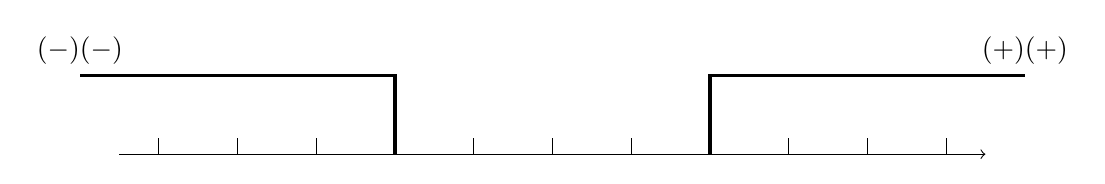
\begin{tikzpicture}
			\draw[->] (-5.5,0)--(5.5,0);
			\foreach \x in {-5,-4,...,5}
			\draw (\x,0.2)--(\x,0);
			\draw[very thick] (-2,0)--(-2,1)--(-6,1) node[above] {$ (-)(-) $};
			\draw[very thick] (2,0)--(2,1)--(6,1) node[above] {$ (+)(+) $};
		\end{tikzpicture}
	\end{figure}

	$$
		x \in (-\infty, 1) \cup \left({10 \over 3}, \infty\right)
	$$
\end{exercise}

\begin{exercise}\nonumber
	Find all values of x that satisfy $ x - 2 \ge {4 \over x+1} $. \\

	\begin{align}
		x - 2                    & \ge {4 \over x+1} \\
		(x-2)(x+1) - 4 \over x+1 & \ge 0             \\
		x^2 - x - 6 \over x + 1  & \ge 0             \\
		(x-3)(x+2) \over x+1     & \ge 0             \\
	\end{align}

	\begin{figure}[H]
		\centering
		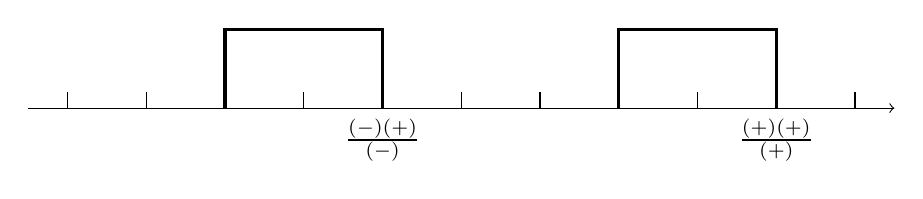
\begin{tikzpicture}
			\draw[->] (-5.5,0)--(5.5,0);
			\foreach \x in {-5,-4,...,5}
			\draw (\x,0.2)--(\x,0);
			\draw[very thick] (-3,0)--(-3,1)--(-1,1)--(-1,0) node[below] {$ {(-)(+)} \over (-) $};
			\draw[very thick] (2,0)--(2,1)--(4,1)--(4,0) node[below] {$ {(+)(+)} \over (+) $};
		\end{tikzpicture}
	\end{figure}

	$$
		x \in [-2, 1) \cup [3, \infty)
	$$
\end{exercise}